
\chapter{Implementation details}\label{chap:implementation-details}

\section{Scala Commander}

Scala Commander is a simple desktop application built as a proof-of-concept for the libraries \emph{Scala.React} and \emph{Scala-Swing}, and for Scala as a language of choice for development of reactive applications.

Scala Commander a \emph{orthodox file manager} application (see figure \ref{fig:scomm_main}). The center of the window consists of two panels (directory lists) each showing the contents of one directory. The user can navigate to an arbitrary directory, can select files and folders, and can execute operations on the selection such as copying, moving, or deletion. The bottom of the window is for file system operations: there is a toolbar with a list of buttons representing file system operations, and whenever a button is clicked, a helper panel appears that prompts the user to confirm the action.

\begin{figure}[h!] 
  \centering
    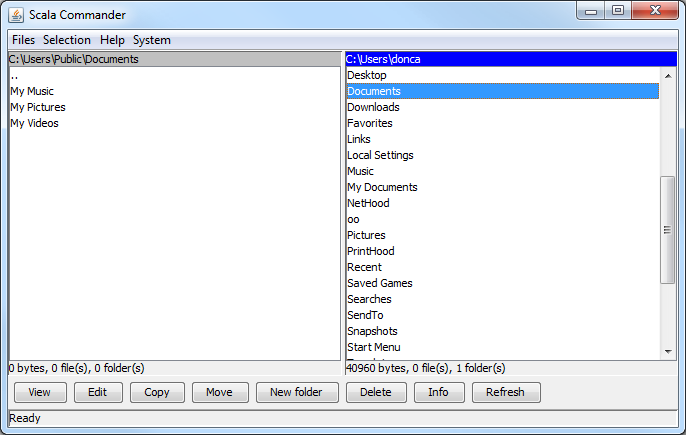
\includegraphics[width=1\textwidth]{images/scala-commander-main.png}
  \caption{Scala-Commander.}
  \label{fig:scomm_main}  
\end{figure}

The user interface is \textbf{constantly reacting to the user input}: as the user selects files and folders, a label always summarizes the selection (shows the number of selected files and folders and the total size of files). File system operations are also reactive: after clicking the \emph{Copy} button, the user can further change the selection (the files and folders to be copied) in the source panel, and can change the destination folder by navigating in the destination panel. Such changes are automatically reflected in the helper panel prompting the user at the bottom of the window. While executing a long-running operation, such as copying, the user interface is not blocked, and the user can always cancel the operation by pressing the \emph{Cancel} button.

The application is built on \emph{Scala.React} and on the the Model-View-Controller design pattern (see section \ref{sec:model-view-controller}): the model consists of \emph{event streams},  \emph{signals} and \emph{reactors}, the view listens to the model signals, and the controller interacts with the model's event streams for simple operations such as navigation, and uses \emph{reactors} for complex operations such as a file system operation.

To demonstrate the design choices, we describes two components in greater detail: the \emph{directory list} and the file system operation \emph{copy}.

\subsection{The directory list}

The main window consists of two directory list components: the \emph{left} list and the \emph{right} list. Both serve the same purpose: the user can see the contents of a directory, can navigate to a subdirectory or to the parent directory, and can select files and folders in the current directory. At any point of time, the directory list that the user last used is the \emph{active} list, while the other list is the \emph{inactive} list. The operations on the toolbar are always executed on the selection of the active list, and the destination of the operation (e.g. copy or move) is the directory of the inactive list.

The design of the implementation is according to the Model-View-Controller design pattern (see figure \ref{fig:mvc_pattern}). The implementation is heavily based on Scala.React concepts, resulting in significantly reduced code length and complexity, as there is no need care for event propagation, dependencies between variables, consistency, and so on.

% The directory list is a list component on the UI that displays the contents of a certain directory. The user can navigate to any subdirectory or can navigate to the parent directory. Navigation automatically updates the list. At any time, the user can select a list of files and folders and do operations on them: copy, move, delete, either by using the buttons on the toolbar or by mouse gesture (drag and drop).

\begin{figure}[h!]
\centering
\begin{tikzpicture} 
\umlemptyclass[x=0, y=-2]{DiskState}
\umlemptyclass[x=3, y=0]{DirectoryListModel}
\umlemptyclass[x=9, y=0]{DirectoryListController} 
\umlemptyclass[x=6, y=-2]{DirectoryListView} 
\umluniassoc[geometry=--]{DirectoryListModel}{DiskState} 
\umluniassoc[geometry=--]{DirectoryListController}{DirectoryListModel} 
\umluniassoc[geometry=--]{DirectoryListController}{DirectoryListView} 
\umluniassoc[geometry=--]{DirectoryListView}{DirectoryListModel} 
\umlVHdep{DirectoryListModel}{DirectoryListView}
\umlHVdep{DirectoryListView}{DirectoryListController}
\umlVHdep{DiskState}{DirectoryListModel}
\end{tikzpicture}
\caption{The directory list components.}
\label{fig:mvc_pattern}
\end{figure}


\subsubsection{Model}

The directory list model (class \texttt{DirectoryListModel}) holds the state of a navigable list and defines a set of operations. The operations alter the internal state of the model (e.g. change the current directory, or change selection). The model is entirely built around Scala.React concepts, such as signal variables, signal functions, event streams and reactors.

The state of the model is defined by the following signal variables:
\begin{itemize}
\item \texttt{currentDirectory: Var[Path]} --- holds the current directory (as a \texttt{java.nio.Path} object);
\item \texttt{selectedPaths: Var[Set[Path]]} --- holds the set of currently selected paths (the selection is highlighted on the user interface);
\item \texttt{active: Var[Boolean]} --- a flag representing whether the directory list is active or inactive;
\item \texttt{diskState: Var[Long]} --- a counter that is incremented whenever the disk is modified and the model need refreshing (u.i. after copying/moving/renaming/deleting, or when the user presses \emph{Refresh}).
\end{itemize}

There are also two derived signals:
\begin{itemize}

\item \texttt{currentDirContents} --- a strict signal that builds the actual list of files and folders that are located inside the current directory; it is dependent on \texttt{currentDirectory} and \texttt{diskState} (the value is just queried and ignored);

\item \texttt{selectionInfo} --- a strict signal holding an aggregated summary of what the user selected, depending \texttt{selectedPaths} and \texttt{currentDirectory}.
\end{itemize}

The model also contains three event sources, each representing an \emph{action} that is defined on the directory list:
\begin{itemize}
\item \texttt{goToParent: EventSource[Unit]} --- go to the parent of the current directory (if it exists);
\item \texttt{goToIndex: EventSource[Int]} --- go to the directory identified by the given index (index of the list \texttt{currentDirContents});
\item \texttt{selectIndices: EventSource[Set[Int]]} --- select paths identified by the given set of indexes.
\end{itemize}

Finally, the model consists of four reactors that glue together the model's state and the event sources: whenever a certain event source emits, they alter the model's state accordingly. The four reactors are the following:
\begin{itemize}
\item \texttt{goToParentReactor} --- awaits the next \texttt{goToParent} event in a loop; when it emits, sets the variable \texttt{currentDirectory} to the parent of the current directory (if it exists);
\item \texttt{goToIndexReactor} --- awaits the next index of \texttt{goToIndex} in a loop; when it emits, sets current directory to the directory identified by the index emitted by the event based on the current value of \texttt{currentDirContents};
\item \texttt{selectIndicesReactor} --- awaits the next index set of \texttt{selectIndices} in a loop; when it emits, sets the variable \texttt{selectedPaths} based on the current value of \texttt{currentDirContents};
\item \texttt{activeReactor} --- awaits the next value of the signal \texttt{active}, and if it is set to false, clears the selection (sets the variable \texttt{selectedPaths} to the empty set).
\end{itemize}

\subsubsection{View}

\begin{wrapfigure}{r}{0.4\textwidth}
  \centering
    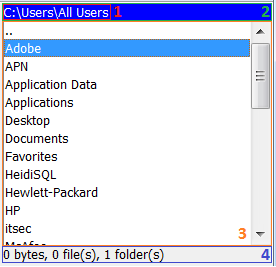
\includegraphics[width=0.35\textwidth]{images/scala-commander-directoryListView.png}
  \caption{The directory list view and its subcomponents.}
  \label{fig:scomm_main}  
\end{wrapfigure}

The directory list view (class \texttt{DirectoryListView}) is responsible for visualizing the model. It is a \texttt{scala.swing.BorderPanel}, and contains four subcomponents (figure \ref{fig:scomm_main}):
\begin{itemize}
\item \texttt{currentDirLabel}: a label displaying the full path of the current directory (marked as \texttt{1});
\item \texttt{currentDirPanel}: the panel containing the label \texttt{currentDirLabel}; the panel's background is blue for the active list and gray for the inactive list (marked as \texttt{2});
\item \texttt{listView}: a \texttt{scala.swing.ListView} component that displays the contents of the current directory, and consists of the \emph{list data} and the \emph{selection} (marked as \texttt{3});
\item \texttt{summaryLabel}: a label displaying a summary of the current selection (marked as \texttt{4}).
\end{itemize}

The view contains \texttt{observe} blocks listening to model signals, where each listener updates the appropriate Swing component. This ensures that the view is always up-to-date as the model changes.

\begin{figure}[h!]
\centering
\begin{lstlisting}[frame=single]
observe(model.currentDirectory) {
  currentDir: Path => currentDirLabel.text = currentDir.toString
}
\end{lstlisting}
\caption{The \texttt{observe} block listening to the changes of the model signal \texttt{currentDirectory}.}
\label{fig:scomm_observe_currentDir}
\end{figure}

The view listens to changes of the following model signals:
\begin{itemize}
\item \texttt{currentDirectory} --- the view updates \texttt{currentDirLabel} (see figure \ref{fig:scomm_observe_currentDir});
\item \texttt{currentDirContents} --- updates the \emph{list data} of \texttt{listView} and clears the \emph{selection};
\item \texttt{selectedPaths} --- updates the \emph{selection} of \texttt{listView};
\item \texttt{selectionInfo} --- updates \texttt{summaryLabel};
\item \texttt{active} --- updates the background of \texttt{currentDirPanel}.
\end{itemize}

\subsubsection{Controller}

The controller (class \texttt{DirectoryListController}) listens to the events of the view's components (extends the trait \texttt{scala.swing.Reactor}), and triggers the appropriate event sources from the model. 

The controller listens to the \emph{mouse clicks}, \emph{selection} and \emph{key} events of the \texttt{listView} component:
\begin{lstlisting}
listenTo(view.listView.mouse.clicks, view.listView.selection, view.listView.keys)
\end{lstlisting}


The controller reacts to the events generated by the above sources as follows:
\begin{lstlisting}
reactions += {
  case MouseClicked(_, _, _, 2, _) => // triggered by `mouse.clicks'
    val leadIndex = view.listView.selection.leadIndex
    model.goToIndex << leadIndex
  case ListSelectionChanged(_, _, false) => // triggered by `selection'
    if (!view.listView.updating) {
      val selection = view.listView.selection.indices.toSet
      model.selectIndices << selection
    }
  case KeyPressed(_, Key.Enter, _, _) => // triggered by `key'
    val leadIndex = view.listView.selection.leadIndex
    model.goToIndex << leadIndex
  case KeyPressed(_, Key.BackSpace, _, _) => // triggered by `key'
    model.goToParent << Unit
}
\end{lstlisting}

Note that the event handling mechanism relies heavily on Scala's pattern matching. For example, in order to listen to double click events, the first case matches events typed of the case class \texttt{MouseClicked} with the fourth parameter \texttt{clicks} fixed to the value \texttt{2}. 

\subsubsection{Interaction between the components}

Figure \ref{fig:scomm_event_propagation} shows the interaction between the components of a directory list when the user changes the current directory. It consists of four stages:
\begin{enumerate}
\item As the user interacts with the UI (double clicks on \texttt{listView}), the event is handled by the controller, and the controller makes event stream \texttt{goToIndex} to emit an index (the index of the line where the double clicked).
\item In the next turn, Scala.React resumes the reactor \texttt{goToIndexReactor}, which gets the index, and queries \texttt{currentDirContents} and \texttt{currentDirectory}, and updates \texttt{currentDirectory} and \texttt{selectedPaths}.
\item In the next turn, Scala.React revalidates the strict signal \texttt{currentDirContents} because its dependency \texttt{currentDirectory} was changed.
\item In the next turn, Scala.React notifies the observer blocks in the view listening to model signals   changed in previous turns; this results in the view components being updated.
\end{enumerate}

\begin{figure}[h!]
\centering
  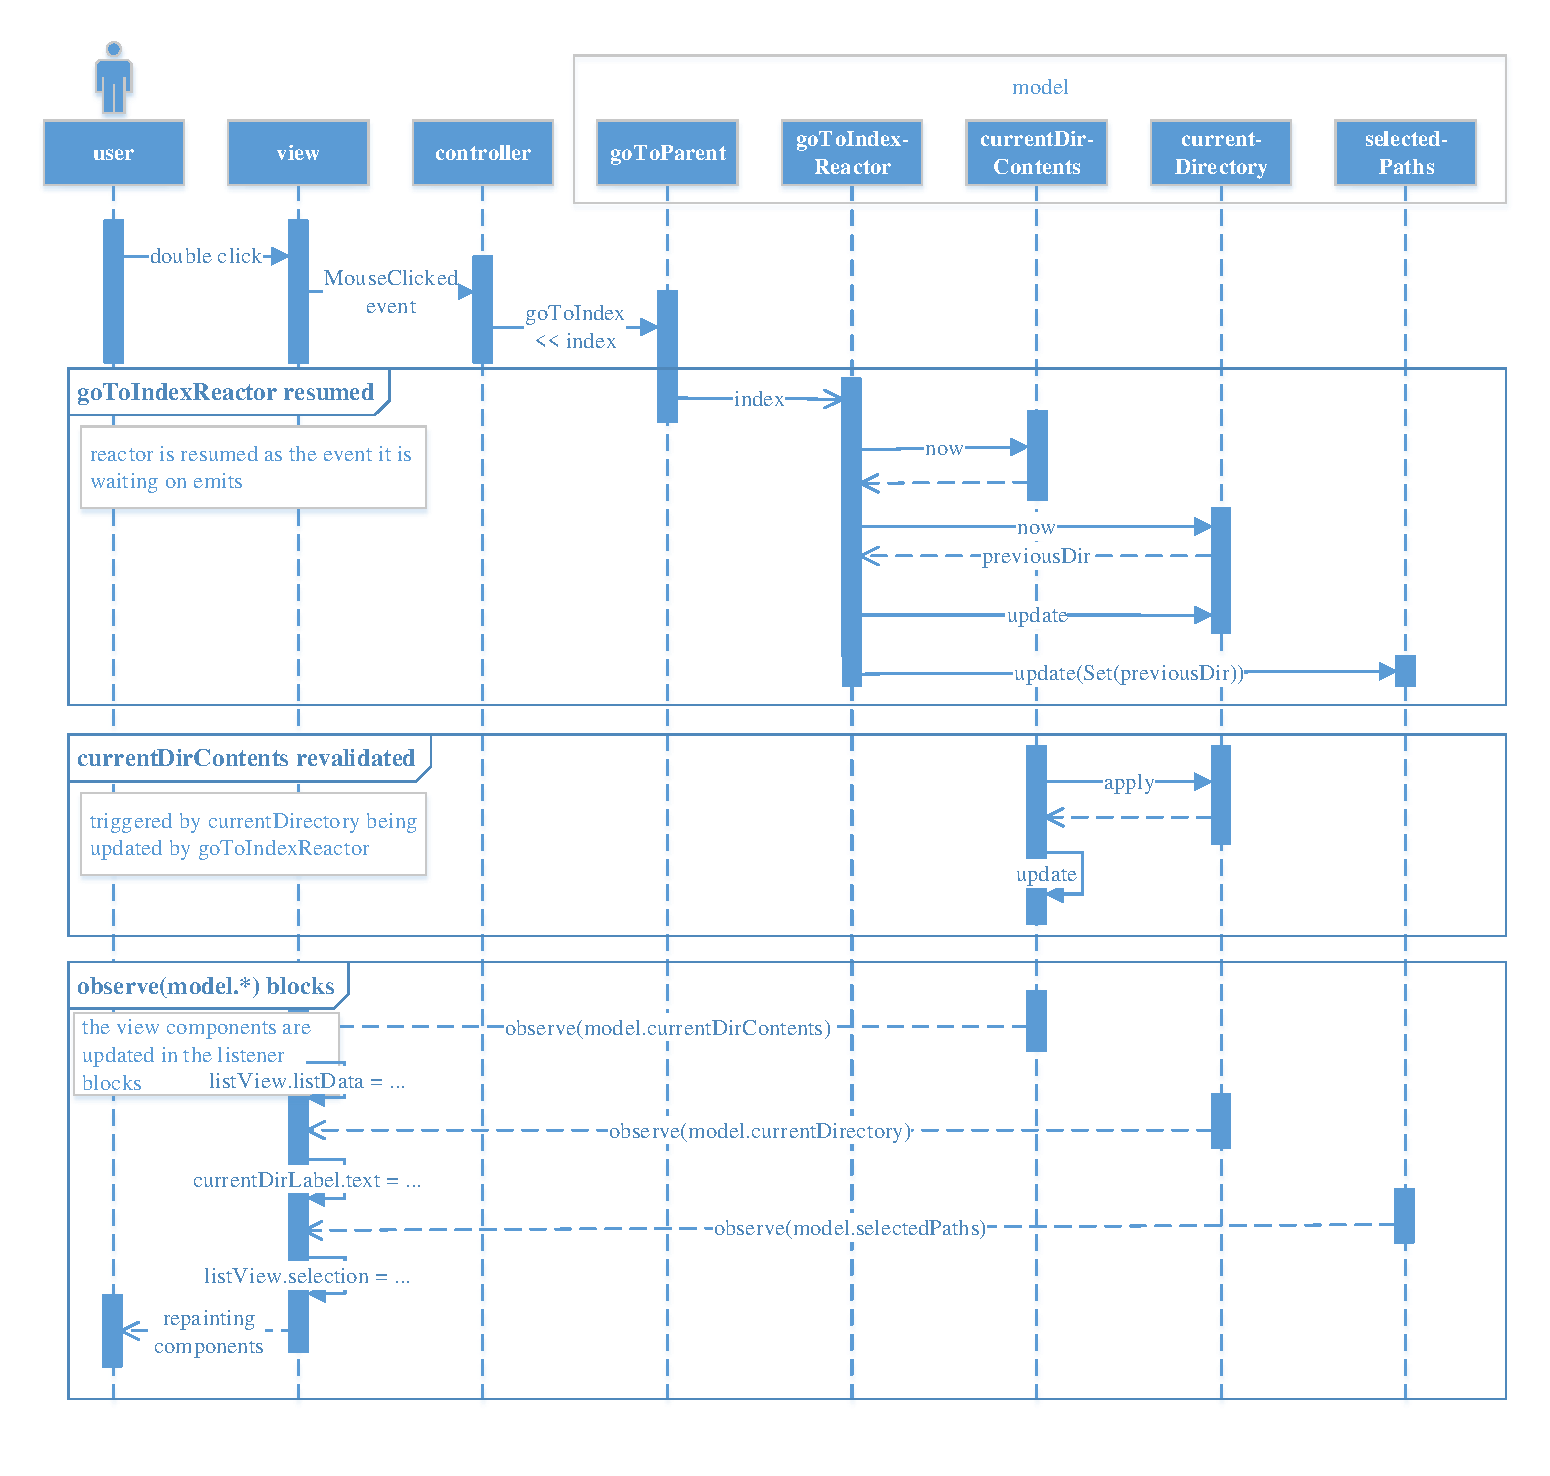
\includegraphics[width=1\textwidth]{images/scomm-event-propagation.pdf}
\caption{Sequence diagram showing the interaction between the components of a directory list when the user navigates in a directory list.}
\label{fig:scomm_event_propagation}
\end{figure}


\subsection{Copying files}

Copying is according to the customs of orthodox file managers: the user selects files and folders in one panel and copies them to the directory where the other panel is navigated to. Traditionally, this is implemented using modal dialogs: once the user clicks a ``Copy'' button, a modal dialog appears prompting him to confirm the action. When confirmed, another modal dialog appears showing the progress of the copying, and until the copying is over, the user cannot interact with the application. 

Our application, however, takes a slightly different approach: when clicking the ``Copy'' button, a panel at the bottom of the window appears. The panel shows the number of files and folders to be copied based on the selection in the active panel, and also contains a text box with the destination path which is the directory of the inactive panel. As the user subsequently navigates the panels, changes the selection, or switches activity, the contents of the panel are automatically updated. Once the user clicks the ``OK'' button in the panel, the selection and the destination directory is captured, and the system beings the copying: the status bar of the window shows the progress, and at any time, the user can abort the operation by pressing the ``Cancel'' button. Copying does not block the application, it remains usable. After copying is done, the directory lists are refreshed.

\subsubsection{Directories pane}

Because copying is defined such as to copy the selection of the \emph{active} list to the directory of the \emph{inactive} list, we need to be able to refer to the active and to the inactive directory list no matter if the left list is active and the right is inactive or vice-versa. This is where the \emph{directories pane} comes into the picture: it consists of the two directory list panels, keeps track of activity based on UI events, and the model has signal functions that always reflect certain properties of the lists. For example, the signal \texttt{activeCurrentDir} always has the value of the active directory list's path, and it is updated when either the user navigates in the active list or switches to the other list.

The model is as follows:

%\begin{figure}[h!]
%\centering

\begin{lstlisting}
class DirectoriesPaneModel(val left: DirectoryListModel,
                                    val right: DirectoryListModel) {

  val activeList = Var[DirectoryListModel]
  val inactiveList = Var[DirectoryListModel]

  val activeCurrentDir = Strict { activeList().currentDirectory() }
  val inactiveCurrentDir = Strict { inactiveList().currentDirectory() }
  val activeSelection = Strict { activeList().selectionInfo() }
  val inactiveSelection = Strict { inactiveList().selectionInfo() }
}
\end{lstlisting}

%\caption{The directories pane model.}
%\label{fig:scomm_directories_pane_model}
%\end{figure}


\subsubsection{Copy controller}

Copying is a single reactor: it awaits the user pressing the \emph{Copy} button on the toolbar, displays the panel, awaits the \emph{OK} button, captures the current state of the directories pane and begins copying. The user can abort the copying by pressing the \emph{Cancel} button at any time. After the copying is done or is aborted, the reactor refreshes the disk state and hides the copy panel.

A simplified version of the reactor code is as follows:

\begin{lstlisting}
Reactor.loop {
  self =>      
    self awaitNext mainWindowView.commandButtons.copyButton()
    
    displayPanel(Some(view.panel)) // display the copy panel
    self.abortOn(view.cancelButton()) { // abort on `Cancel'
      self awaitNext view.okButton() // wait until `OK'

      val sources: Set[Path] = directoriesPane.activeSelection.now.paths
      val destinationDir: Path = directoriesPane.inactiveCurrentDir
      sources.cps foreach { // do the copying
        ... self pause ... // for `abortOn' to be able to abort the copying
      }
    }
    diskState.refresh()
    displayPanel(None) // hide the copy panel
}
\end{lstlisting}


Note that the \texttt{abortOn} operator executes the body and aborts it as soon as the given reactive (the cancel button) emits. This makes it possible to cancel while waiting for the \emph{OK} button or while actually copying the files.




\section{FEST-Logging}\label{sec:test-auditing}

Test suites testing even relatively complex applications can easily contain some hundred tests. Because UI tests, by their nature, typically take much time, the total run time of an entire test suite is usually important. In order to keep the overall runtime at minimum, it is typical to avoid the creation, initialization and the destruction of the individual UI components for each test (which might also be difficult or impossible depending on the architecture of the application). A possible option is to test entire applications and to reuse the same components between the tests.

The problem with testing entire applications throughout entire test suites is that the tests can become dependent on the internal state of the application and on the state of the UI. Thus, it is possible for one test to affect the outcome of another, e.g. one test makes a subtle change in the state of the application and makes another test fail, or, in a more extreme case, one failing test can leave the application in such a state that no other further tests will pass. Having non-independent tests can lead to fragile and unstable test systems and thus should be avoided as much as possible.

Unstable test system can very difficult to cope with. Tests can seemingly fail randomly, and it can be very difficult to reproduce failures that originate from typically a subtle change in the application's state that was made by a previous test (possibly executed many tests before). FEST supports saving screenshots anytime during a test, but the test must explicitly save it and it is usually done only on errors. Since in the case of unstable tests, the errors typically manifest themselves only in the tests that are affected by the erroneous tests' side effects, saving screenshots for failing tests does not help much on its own.

Understanding the data flow of all the tests of an entire test suite, knowing all the operations that were made on the application's state, along with screenshots made after all important steps can greatly reduce the debugging efforts of an unstable test suite and can benefit the test development and maintenance process.

\subsection{FEST-Logging: AspectJ-based auditing}

We introduce \emph{FEST-Logging}, an AspectJ-based solution that gathers information of the test methods and on annotated methods in the user code. The gathered information (method arguments, screenshots) are visualized in the form of a table and the entire execution tree can be inspected.

We introduce the JUnit runner \texttt{CacioFESTLoggingRunner}: enables FEST-Logging and executes the tests using the \emph{Cacio-tta} graphics stack (running the tests in the background). Running the tests with this runner is a \textbf{requirement} of FEST-Logging.

We also introduce two annotations:
\begin{itemize}
\item \texttt{GUITestBean}: a \emph{type} annotation
\item \texttt{GUITestAction}: a \emph{method} annotation.
\end{itemize}

FEST-Logging provides the following features:
\begin{itemize}
\item auditing tests --- audits the \emph{test}, \emph{setup} and \emph{teardown} methods (annotated with \texttt{@Test}, \texttt{@Before} and \texttt{@After}).
\item auditing test actions --- audits \emph{all} methods of classes annotated with \texttt{@GUITestBean};
\item screenshots of test actions --- the runtime system takes screenshots \emph{before} and \emph{after} methods annotated with \texttt{@GUITestAction} are executed;
\item screenshots of failed tests --- the runtime system takes screenshots of failing tests, failing either in their \emph{test}, \emph{setup} or \emph{teardown} methods. 
\end{itemize}

Tests using FEST-Logging generate reports as files in the folder \emph{reports/xml}. The reports can be visualized using the HTML page \emph{web/report.html}.

\subsection{Implementation}

Using a JUnit runner lets us add additional behavior to the execution of a test, similarly to advices in AspectJ. The runner \texttt{CacioFESTLoggingRunner} takes this opportunity to register the test in the object \texttt{MethodCallStack} and to execute the test. When the test is over, it captures any exceptions thrown by the test, unregisters the test from \texttt{MethodCallStack} and writes the audited data to the reports folder.

The test methods and test actions are altered by the aspect class \texttt{FESTLoggingAspect}. Here, we define a series of pointcuts, where each pointcut is to match a method annotated with a certain annotation (see figure \ref{fig:fest-logging-pointcuts}). There are also \emph{around advices} defined referring to the pointcuts, where each advice alters the execution of the method:
\begin{itemize}
\item \texttt{auditTestAndGUITestBeanMethods} --- registers and gathers the result of the advised method;
\item \texttt{takeScreenshotOfFailedTest} --- advises test methods, and takes screenshots if they throw exceptions;
\item \texttt{takeScreenshotsOfTestActions} --- takes screenshots \emph{before} and \emph{after} executing the advised method.
\end{itemize}
Each advice relies on the object \texttt{MethodCallStack}, and stores the gathered data in it.

\begin{figure}[h!]
\centering
\begin{lstlisting}
@Aspect
class FESTLoggingAspect {
  @Pointcut("execution(@org.junit.Test * *.*(..))")
  def testMethods() {}

  @Pointcut("execution(@org.junit.Before * *.*(..))")
  def beforeMethods() {}

  @Pointcut("execution(@org.junit.After * *.*(..))")
  def afterMethods() {}

  @Pointcut("execution(* (@edu.zsd.festlogging.GUITestBean *).*(..))")
  def guiTestBeanMethods() {}

  @Pointcut("execution(@edu.zsd.festlogging.GUITestAction * *.*(..))")
  def guiTestActionMethods() {}
  ...
}
\end{lstlisting}
\caption{The pointcuts matching to test methods (first three) and to test actions (last two).}
\label{fig:fest-logging-pointcuts}
\end{figure}

\subsubsection{Test auditing: building the method stack}

Figure \ref{fig:fest-logging-auditMethods} shows the advice responsible for auditing. It calls the method \texttt{enterTestMethod}, proceeds the join point, and finally calls the \texttt{exitTestMethod}. This is so the class \texttt{MethodCallStack}, as the name suggests, can keep a stack of objects representing the advised methods.

\begin{figure}[h!]
\centering
\begin{lstlisting}
  @Around("testMethods() || beforeMethods() || afterMethods() || guiTestBeanMethods()")
  def auditMethods(joinPoint: ProceedingJoinPoint): AnyRef = {
    MethodCallStack.enterTestMethod(joinPoint)
    try {
      val result: AnyRef = joinPoint.proceed()
      MethodCallStack.exitTestMethod(joinPoint, result)
      result
    } catch {
      case e: Throwable =>
        MethodCallStack.exitTestMethod(joinPoint, e)
        throw e
    }
  }
\end{lstlisting}
\caption{The pointcuts matching to test methods (first three) and to test actions (last two).}
\label{fig:fest-logging-auditMethods}
\end{figure}

The class \texttt{MethodCallStack} holds a single reference named \texttt{current} of type \texttt{RunningExecution} (see figure \ref{fig:fest-logging-MethodCallStack}). This represents the \emph{top} of the stack. The very first running execution object is pushed into the stack by \texttt{CacioFESTLoggingRunner} in the form of a \texttt{RunningTestExecution} object. The class \texttt{RunningExecution} holds the advised method, the argument list, has a mutable list of child method invocations and mutable screenshot fields. 

Subsequently, when the actual test methods and the test action methods are executed, the advice \texttt{auditMethods} pushes a new \texttt{RunningTestMethodExecution} object with the parent reference set to the top of the stack. When a method terminates, the stack is ``popped'': the top object, referenced by \texttt{current}, is converted into a new \texttt{Execution} object, this \texttt{Execution} object is added to the invocation list of its parent, and this parent is then assigned to the variable \texttt{current}.

\begin{figure}[h!]
\centering
  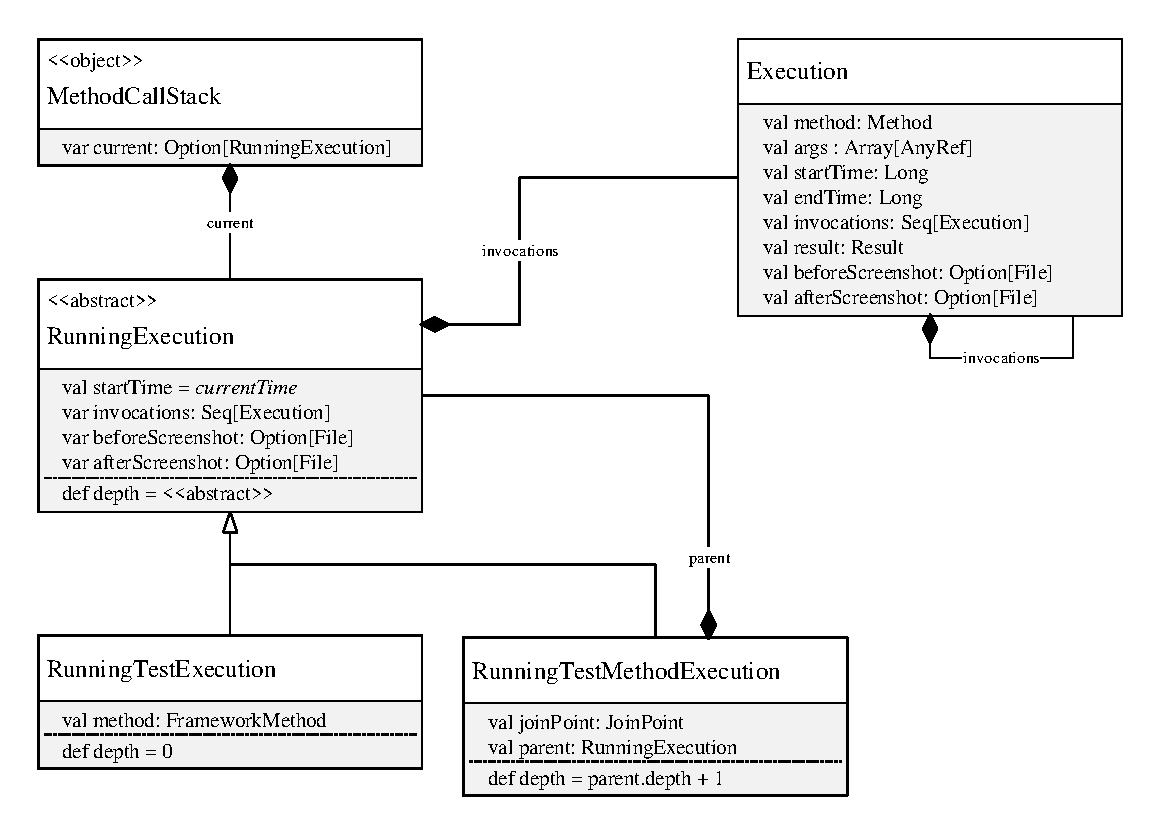
\includegraphics[width=1\textwidth]{images/FESTLogging-MethodCallStack.pdf}
\caption{Class diagram of the classes internally used by the object \texttt{MethodCallStack}. Class \texttt{RunningExecution} represents an ongoing execution (with mutable fields), and the class \texttt{Execution} represents a terminated execution (with immutable fields).}
\label{fig:fest-logging-MethodCallStack}
\end{figure}

When the execution reaches back the class \texttt{CacioFESTLoggingRunner}, the variable \texttt{current} \textbf{must be} referencing to a \texttt{RunningTestExecution} object. This also transformed to an \texttt{Execution} object, but instead of further pushing it on the stack, this object is transformed to XML format and is written to the reports folder.

\subsubsection{Taking screenshots}

There are two advices taking screenshots: \texttt{take\-Screen\-shot\-Of\-Failed\-Test} and \texttt{take\-Screen\-shots\-Of\-Test\-Actions}. Both rely on the object \texttt{MethodCallStack}: they take the topmost \texttt{Running\-Execution} object on the stack, take the screenshots into files and assign the appropriate fields in the \texttt{Running\-Execution} object. This is based on AspectJ applying multiple advices on the same method using well-defined precedence rules (which is declaration precedence in this case).

\subsection {Formatting the audited data}

Since the runtime data set can be huge for long tests runs, it is important to provide views that presents the data in an easily accessible, intuitive and adaptive form. 

A possible implementation is to generate an HTML page that contains all the data in the form of a pivot table, with a tree axis showing the call hierarchy, and the columns presenting the method arguments and other context info. The pivot table would support drill-down in the call hierarchy. This table would support the following:
\begin{itemize}
\item Closing and expanding nodes (method calls) in the call hierarchy;
\item Filtering and sorting by the context data (e.g. method names, arguments, annotations).
\end{itemize}

The following is a simple example of a test of a text editor application consisting of the following steps:
\begin{itemize}
\item create a new text file
\item enter the text ``hello'' and `` world'', respectively
\item save the text file to the disk
\item assert that the editor shows the file name in the window's title
\item assert that the file exists on the disk and has the appropriate content
\end{itemize}

Table \ref{fig:formatted_audited_data_report} shows the method calls only of the test, user action and adapter layers, along with the arguments and the return values (if applicable).

\begin{table}
\caption{Formatted audited data report}
%\rowcolors{2}{gray!25}{white}
\begin{tabular}{l l c}
%\rowcolor{gray!50}
\hline\hline

Method call & Arguments & Returns \\ [0.5ex] % inserts table heading
\hline 

\hskip 0cm EditorTest.saveNewTextFile & & PASSED \\
\hskip 3mm   EditorUserActions.createNewTextFile & & \\
\hskip 6mm     MenuAdapter.clickFileMenu & & \\ 
\hskip 6mm     MenuAdapter.clickNewTextFileMenuItem & & \\ 
\hskip 3mm   EditorUserActions.enterText & text=''hello'' & \\
\hskip 6mm     TextAreaAdapter.getCaretPosition & & 0 \\
\hskip 6mm     TextAreaAdapter.insertText & position=0, text=''hello'' & \\
\hskip 3mm   EditorUserActions.enterText & text=''world'' & \\
\hskip 6mm     TextAreaAdapter.getCaretPosition & & 5 \\
\hskip 6mm     TextAreaAdapter.insertText & position=5, text='' world'' & \\
\hskip 3mm   EditorUserActions.saveCurrentEditor & filename=''C:{\textbackslash}helloWorld.txt'' & \\
\hskip 6mm     MenuAdapter.clickFileMenu & & \\
\hskip 6mm     MenuAdapter.clickSaveMenuItem & & \\
\hskip 6mm     DialogAdapter.setFileName & filename=''C:{\textbackslash}helloWorld.txt'' & \\
\hskip 6mm     DialogAdapter.clickSaveButton & & \\
\hskip 6mm     DialogAdapter.expectToDisappear & & \\	 
\hskip 3mm   EditorUserActions.expectTitle & title=''helloWorld'' & \\
\hskip 6mm     MainWindowAdapter.expectTitle & title=''My Notepad - helloWorld'' & \\
\hskip 6mm     FileUtils.expectFileContents &
    \begin{tabular}[x]{@{}c@{}}
       path=''C:{\textbackslash}helloWorld.txt", \\
      contents=''hello world''
    \end{tabular} & \\

\hline

\end{tabular}
\label{fig:formatted_audited_data_report}
\end{table}

\subsection{Automatic EDT dispatch}\label{sec:edt-dispatch}

The threading model of Swing recommends that all Swing-component-related operations are to be executed on the Swing EDT thread, including those of the tests. It is the test developer's responsibility to respect this rule, and thus to delegate all such work to the EDT thread. There are two options: one can either use \texttt{Swing\-Utilities.invoke\-And\-Wait}, or can use the more convenient class \texttt{GuiActionRunner} offered by FEST-Swing. This, in either case, leads to much boilerplate code in the adapter layer and is error-prone.

To offer a solution to this problem, we present the annotation \texttt{ExecuteInEDT} (part of \emph{FEST-Logging} library). When an annotated method is called on the test thread, the method is seamlessly and transparently delegated to the Swing EDT thread, and the test thread awaits the result (the return value or the exception). This leads to less effort from the developer's side, and at the same time, increases security on the tests' correctness.

\subsubsection{Implementation}\label{sec:edt-dispatch}

We define a pointcut that matches methods annotated with \texttt{ExecuteInEDT}, and we use an \emph{around advice} to delegate the invocation to Swing EDT:
\begin{lstlisting}
@Pointcut("execution(@edu.zsd.festlogging.ExecuteInEDT * *.*(..))")
def executeInEDTMethods() {}

@Around("executeInEDTMethods()")
def executeInEDT(joinPoint: ProceedingJoinPoint) : AnyRef = {
  GuiActionRunner.execute(new GuiQuery[AnyRef] {
    override def executeInEDT(): AnyRef = joinPoint.proceed()
  })
}
\end{lstlisting}

The method \texttt{GuiActionRunner.execute} takes a single \texttt{query} argument and executes it on Swing EDT. If the current thread is already Swing EDT, the method directly executes the argument and returns the value, otherwise it uses \texttt{SwingUtilities.invokeLater} to execute the method and wait for the response. In case the method threw an exception, the stack trace is \textbf{merged} with the invocation stack of the \texttt{GuiActionRunner.execute} method, resulting in an exception that looks just as if the query was executed synchronously on the test thread.

\subsection{Simulated drag-and-drop}\label{sec:simulated-dnd}

\subsubsection{Defective DnD with Cacio-tta}\label{sec:defective-dnd}

FEST-Swing completely supports mouse gesture-based drag-and-drop (DnD) between Swing components, allowing the tests to cover that part of the application's functionality. However, some limitations (see above \fullref{sec:fest-swing-limitations}) often required the tests system to use the alternative graphics stack implementation named Cacio-tta \cite{Cacio_Tta_FEST} with the known limitation that it does not provide the required system-level support for drag and drop. Thus, in such test systems the mouse gesture-based approach of FEST-Swing's does not work.

A solution would be to programmatically trigger the data export and import operations on the Swing components, thus simulating the drag and drop without any mouse movement. However, because of the platform-dependent nature of the Swing (and AWT) DnD subsystem \cite{IntroDnD} \cite{DnDSubsystem}, this is not trivial to be realized.

\subsubsection{Drag and drop in Swing - Behind the scenes}\label{sec:dnd-swing}

Let us say that the user, who is running a Java application, wants to drag some text from a list and deposit it into a text field. Briefly, the drag and drop process consists of the following steps \cite{IntroDnD}:

\begin{enumerate}
\item The user has selected a row of text in the source component: the list. While holding the mouse button the user begins to drag the text - this initiates the drag gesture.
\item \label{item:drag-begin} When the drag begins, the list component packages up the data for export and declares what source actions it supports (i.e. COPY, MOVE, or LINK).
\item As the user drags the data, Swing continuously calculates the location and handles the rendering.
\item If the user simultaneously holds the Shift and/or Control key during the drag, this user action is also part of the drag gesture. Typically, an ordinary drag requests the MOVE action. Holding the Control key while dragging requests the COPY action, and holding both Shift and Control requests the LINK action.
\item \label{item:insert-location} Once the user drags the text over the bounds of a text field component, the target is continually polled to see if it will accept or reject the potential drop. As he drags, the target provides feedback by showing the insert location, perhaps an insertion cursor or a high-lighted selection. In the current example, the text field (the current target) allows both re-placement of selected text and insertion of new text.
\item \label{item:import-data} When the user releases the mouse button, the text component imports the data by inspecting the declared source actions and any user action and then it chooses what it wants out of the available options. In the current example, the text field chooses to insert the new text at the point of the drop.
\end{enumerate}

While this might seem like a daunting process, Swing handles most of the work out of the box. The Swing framework is designed so that the developer plug in the details specific to the components, and the rest is automatic.

\subsubsection {Simulated drag-and-drop}\label{sec:simulated-dnd}

By doing the following steps, the tests can programmatically trigger drag-and-drop:
\begin{enumerate}
\item Trigger an export on the source component (see point \ref{item:drag-begin} above).
\item Set the proper insert location at the destination component (see point \ref{item:insert-location} above).
\item Trigger the import of the data (see point \ref{item:import-data} above).
\end{enumerate}











